\documentclass[12pt]{article}

\usepackage{amsmath}
\usepackage{graphicx}
\usepackage{dcolumn}
\usepackage{booktabs}
\usepackage{rotating}
\usepackage{subcaption}
\usepackage{listings}
\usepackage{multirow}

\usepackage{setspace}
\usepackage{parskip}
\usepackage[top=1in,bottom=1in,left=1in,right=1in]{geometry}

\usepackage{natbib}
\usepackage[pdfstartpage=1,pdfpagemode=UseNone,pdfstartview=FitH,pdffitwindow=true,bookmarks=false,colorlinks=true,linkcolor=blue,citecolor=blue]{hyperref}

% define lightgray
\usepackage[table]{xcolor}
\definecolor{lightgray}{gray}{0.9}

\begin{document}


%%%%%%%%%%%%%%%%%%%%%%%%%%%%%%%%
% Tables
%%%%%%%%%%%%%%%%%%%%%%%%%%%%%%%%
{\bf Title:} Descriptives \\
{\bf Authors:} Jonathan P. Latner \\
{\bf Revision date:} \today

\begin{table}[htbp]
\centering
\caption{Comparison of Baseline and Tuned Parameters}
\begin{tabular}{|c|c|c|c|c|}
\hline
\textbf{Model} & \textbf{Parameter} & \textbf{Baseline} & \textbf{Tuned} & \textbf{Different} \\ \hline
\multirow{3}{*}{Synthpop}   & cp            & 0.00000001    & 0.00000001& Y \\                            & minbasket     & 5             & 5         & Y \\ 
                            & copies (m)    & 1             & 10        & N \\ \hline
\multirow{5}{*}{CTGAN}      & epochs            & 300   & 900   & Y \\ 
                        & discriminator steps   & 1     & 10    & Y \\ 
                        & batch size            & 500   & 500   & N \\ 
                        & log frequency         & FALSE & FALSE & N \\ 
                        & copies (m)            & 1     & 10    & N \\ \hline
\multirow{4}{*}{DataSynthesizer} & privacy (e)  & 0.1   & 30    & Y  \\ 
                        & parents (k)           & 0     & 1     & Y  \\ 
                        & copies (m)            & 1     & 10    & Y  \\ \hline
\end{tabular}
\end{table}


\begin{table}[!h]
    \caption{Utility - baseline}
    \centering
    \resizebox{.8\textwidth}{!}{% latex table generated in R 4.3.0 by xtable 1.8-4 package
% Wed Aug  9 17:01:02 2023
\begin{tabular}{lrrr}
  \toprule
Metric & Synthpop & DataSynthesizer & CTGAN \\ 
  \midrule
\medskip ROE univariate & 0.9784 & 0.9381 & 0.8786 \\ 
  CI Overlap & 0.7910 & 0.4865 & 0.4725 \\ 
  Standardized difference & 0.8192 & 2.0085 & 2.1922 \\ 
   \bottomrule
\end{tabular}
}
    \label{table_utility_baseline}
\end{table}

\begin{table}[!h]
    \caption{Utility - tuned}
    \centering
    \resizebox{.8\textwidth}{!}{% latex table generated in R 4.3.0 by xtable 1.8-4 package
% Wed Aug  9 17:01:05 2023
\begin{tabular}{lrrr}
  \toprule
Metric & Synthpop & DataSynthesizer & CTGAN \\ 
  \midrule
\medskip ROE univariate & 0.9829 & 0.9807 & 0.9681 \\ 
  CI Overlap & 0.8667 & 0.8558 & 0.8144 \\ 
  Standardized difference & 0.5406 & 0.5635 & 0.7252 \\ 
   \bottomrule
\end{tabular}
}
    \label{table_utility_tuned}
\end{table}

\begin{figure}[!h]
    \centering
    \caption{Frequency of estimates}
    \resizebox{\textwidth}{!}{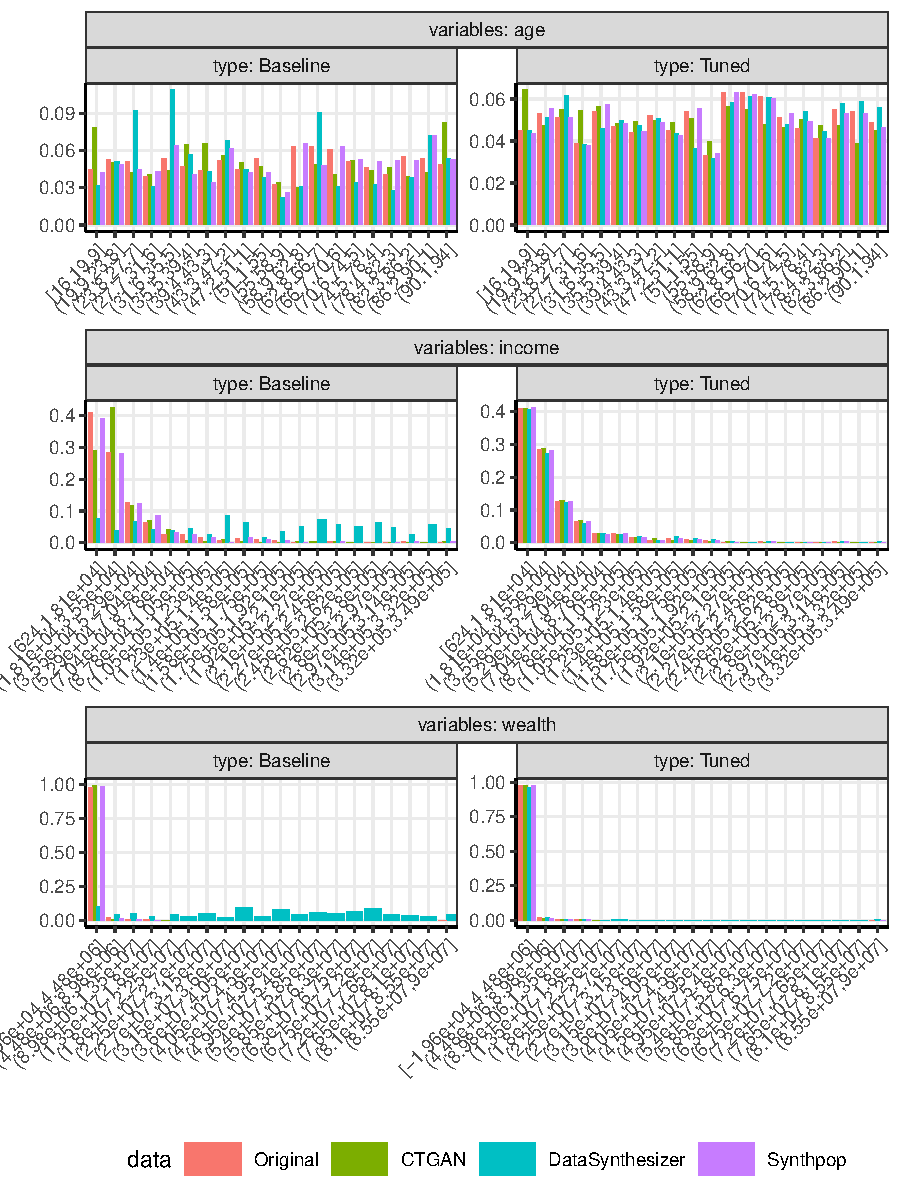
\includegraphics{../graphs/graph_compare_frequency.pdf}}
    \label{graph_compare_frequency}
\end{figure}

\begin{figure}[!h]
    \centering
    \caption{Confidence interval overlap}
    \resizebox{\textwidth}{!}{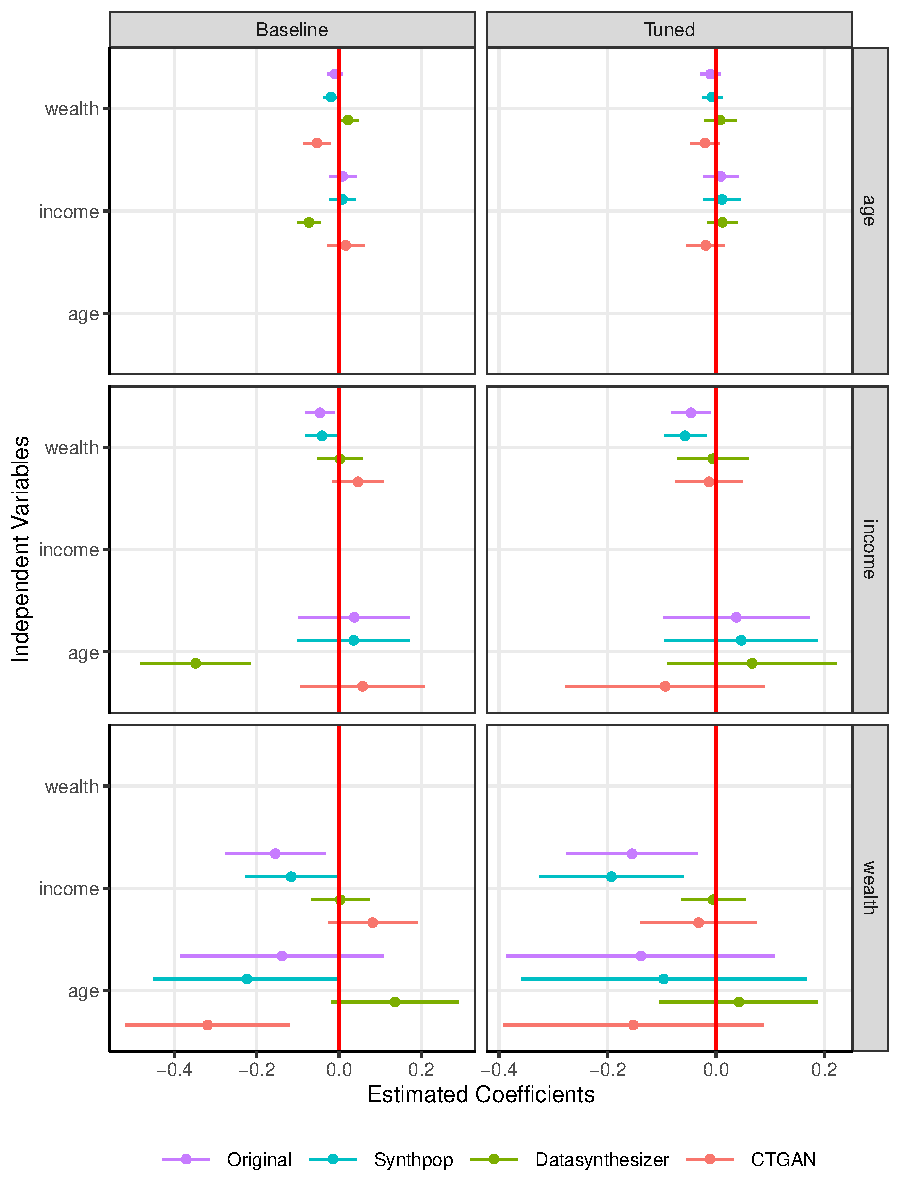
\includegraphics{../graphs/graph_compare_cio_regressions.pdf}}
    \label{graph_compare_cio_regressions}
\end{figure}

\end{document}

